\newcommand{\texCommand}[1]{\texttt{\textbackslash{#1}}}%

\newcommand{\exemplo}[1]{%
\vspace{\baselineskip}%
\noindent\fbox{\begin{minipage}{\textwidth}#1\end{minipage}}%
\\\vspace{\baselineskip}}%

\newcommand{\exemploVerbatim}[1]{%
\vspace{\baselineskip}%
\noindent\fbox{\begin{minipage}{\textwidth}%
#1\end{minipage}}%
\\\vspace{\baselineskip}}%

Este capítulo descreve toda a fundamentação teórica por trás das tecnologias utilizadas na implementação do estudo de caso. Inicialmente, explico os conceitos gerais relacionados a teoria de grafos, em seguida, aponto as principais características e utilidades dos SGBDs NoSQL. Posteriormente, aponto as características e particularidades de um SGBD orientado a grafos, junto com uma explicação acerca do SGBD escolhido para o trabalho que é o OrientDB. Por fim, explico um pouco sobre a tecnologia REST utilizada para a comunicação entre o sistema desenvolvido e o OrientDB.

%%%%%%%%%%%%%%%%%%%%%%%%%%%%%%%%%%%%%%%%%%%%%%%%%%%%%%%%%%%%%%%%%%%%%%%%%%%%%%%%
%%%%%%%%%%%%%%%%%%%%%%%%%%%%%%%%%%%%%%%%%%%%%%%%%%%%%%%%%%%%%%%%%%%%%%%%%%%%%%%%
%%%%%%%%%%%%%%%%%%%%%%%%%%%%%%%%%%%%%%%%%%%%%%%%%%%%%%%%%%%%%%%%%%%%%%%%%%%%%%%%
\section{Teoria de Grafos}



%%%%%%%%%%%%%%%%%%%%%%%%%%%%%%%%%%%%%%%%%%%%%%%%%%%%%%%%%%%%%%%%%%%%%%%%%%%%%%%%
%%%%%%%%%%%%%%%%%%%%%%%%%%%%%%%%%%%%%%%%%%%%%%%%%%%%%%%%%%%%%%%%%%%%%%%%%%%%%%%%
%%%%%%%%%%%%%%%%%%%%%%%%%%%%%%%%%%%%%%%%%%%%%%%%%%%%%%%%%%%%%%%%%%%%%%%%%%%%%%%%
\section{SGBD NoSQL}
	Essa seção aborda a categoria de bancos de dados não relacionais. Inicialmente, realizo uma introdução sobre o assunto, para em seguida explicitar as principais características e categorias dentro desse grupo de bancos de dados.
	
\subsection{Introdução}
	O termo NoSQL foi utilizado na literatura pela primeira vez por Carlo Strozzi em 1998 como o nome de um banco de dados que ele estava desenvolvendo na época \cite{FirstNoSQL}. Curiosamente, é um banco relacional que não possuia interface SQL, portanto, NoSQL. Entre o período dos anos de 2000 e 2005 o universo dos SGBD NoSQL começou a aumentar bastante, o SGBD baseado em grafo Neo4j começou a ser desenvolvido no ano de 2000, o SGBD da Google BigTable\cite{Chang:2008:BDS:1365815.1365816} começa em 2004 e em seguida o CouchDB se inicia por volta de 2005. Porém, todas essas tecnologias não eram na época categorizadas como NoSQL, somente em 2009 o termo foi reintroduzido por Johan Oskarsson ao organizar um evento para discutir sobre banco de dados não relacionais, distribuídos e de código aberto, e a partir desse momento o termo passa a ser usado para categorizar os bancos de dados não relacionais.
	
	O termo NoSQL gera muita confusão pois leva a entender que os bancos de dados nessa categoria não utilizam a linguagem SQL. Porém, o termo costuma ser utilizado como \textit{Not only SQL}, e demonstra que tais sistemas podem suportar também linguagens de consultas baseadas em SQL. O aspecto mais importante por trás dos SGBD NoSQL é o motivo de seus surgimentos. No início dos anos 2000, a forma como os usuários começaram a interagir na internet começou a evoluir e consequentemente os sistemas e aplicações passaram a gerar e consumir cada vez mais dados e informações. Esse crescimento na geração e consumo de dados foi enorme, e por isso os especialistas necessitavam de tecnologias que atendessem melhor suas necessidades, desse cenário começaram a nascer os primeiros SGBD NoSQL como o BigTable da google e o Dynamo da Amazon\cite{DeCandia:2007:DAH:1323293.1294281}.
	
\subsection{Características de um SGBD NoSQL}
	Como foi mencionado acima, por volta dos anos 2000 começou a nascer a necessidade de novas tecnologias na área de banco de dados. Os sistemas precisavam de boa escalabilidade horizontal para operações de forma distribuída, entre outras coisas. Vários aspectos relacionados a categoria dos SGBD NoSQL são ainda abertos e não possuem um consenso. O trabalho feito por Rick Cattell\cite{Cattell:2011:SSN:1978915.1978919} aglomerou algumas características que geralmente se encontram nesse tipo de banco de dados: 
	\begin{itemize}
		\item Habilidade de escalar horizontalmente operações simples através de vários servidores
		\item Habilidade de replicar e distribuir os dados através de vários servidores
		\item Um modelo de concorrência mais flexível que as transações ACID presentes em sistemas relacionais.
		\item Uso eficiente de índices distribuidos e da memória RAM para armazenar os dados
		\item Habilidade de adicionar dinamicamente novos atributos a um registro
	\end{itemize}
	
	Porém, é importante ressaltar que nem todas essas características precisam ser atendidas para fazer parte dessa categoria. Sendo que também existem outras características importantes observadas em alguns sistemas como por exemplo, disponibilidade e consistência dos dados, níveis de flexibilidade para o esquema do banco de dados e etc.

\subsection{Gerenciamento de Transações} \label{manage_transaction}
	Uma propriedade importante em qualquer SBGD é o controle de concorrência. Normalmente, vários usuários solicitam operações ao SGBD simultâneamente, sendo que esse sistema gerenciador de banco de dados precisa garantir aos usuários a integridades dos dados transacionados. A maioria dos bancos de dados relacionais utilizam transações ACID\cite{SistemaDeBd} para controlar essa concorrência, que impõe ao SGBD as seguintes propriedades:
	\begin{itemize}
		\item Atomicidade: Essa propriedade impôe que durante uma transação, todas as alterações feitas no banco de dados sejam efetivadas. Caso ocorra algum erro durante a transação o SGBD realiza um \textit{rollback} para o estado consistente anterior a transação.
		\item Consistência: Essa propriedade impôe que ao término de uma transação o banco de dados está de forma consistente. Ou seja, a cada transação os dados devem estar consistentes e a garantia de que as restrições impostas aos dados não sejam violadas.
		\item Isolamento: A propriedade de isolamento de uma transação, busca impor ao SGBD que cada transação seja independente das demais. Ou seja, garante que cada transação seja vista como uma unidade e impede que outras transações acessem dados que possam levar o bancos de dados a um estado inconsistente. 
		\item Durabilidade: A durabilidade garante que as informações salvas após cada transação permaneçam no banco de dados. Os dados não podem desaparecer em nenhum momento e devem permanecer persistidos independente de qualquer falha.
	\end{itemize}
	
	Esse formato é utilizado por bancos de dados relacionais, e atende bem uma boa parte de sistemas e aplicações nos dias de hoje, como é o caso de sistemas bancários por exemplo, que necessitam dessas propriedades para garantir a integridades das informações de seus clientes.
	
	O mais importante a se perceber aqui é que nem toda aplicação precisa necessariamente desse controle de concorrência elaborado. No caso de bancos é de suma importância esse tipo de controle, agora em uma aplicação de alta disponibilidade uma propriedade como a consistência pode ser um pouco mais fraca. Portanto, para atender a essas novas demandas, nasceu o modelo de transações BASE\cite{Pritchett:2008:BAA:1394127.1394128} que busca fornecer maior flexibilidade para esses novos sistemas. O BASE tem como característica em vez de exigir consistência após cada transação, é suficiente para o banco de dados estar eventualmente consistente. Existe um teorema famoso feito por Eric Brewer conhecido como Teorema CAP\cite{Brewer:2010:CFT:1835698.1835701}, que demonstra o trade-off entre consistência, disponibilidade e tolerância a particionamento. Eric diz que se for necessário essas três características, é necessário escolher somente duas delas. Portanto no modelo BASE é possíve escolher tolerância a particionamento e disponibilidade e abrir mão de uma alta consistência dos dados. O acrônimo BASE vem das três seguintes características:
	\begin{itemize}
		\item \textit{Basic Availability}: Essa propriedade no fundo quer dizer que o banco de dados aparenta funcionar a maior parte do tempo.
		\item \textit{Soft state}: Essa propriedade quer dizer que as bases não precisam estar sempre consistentes, nem as réplicas precisam estar consistentes o tempo inteiro. Ou seja, o estado do sistema é volátil.
		\item \textit{Eventual consistency}: Essa propriedade diz que as bases de dados vão ficar eventualmente consistentes no futuro. 
	\end{itemize}
	
\subsection{Categorias de NoSQL}
	Dentro do universo dos SGBD NoSQL, existem cinco grandes categorias que separam cada SGBD em relação a estratégia de armazenamento\cite{nayak2013type}. Tais categorias são:
	
\subsubsection{SGBD NoSQL por chave/valor}
	Os SGBD dessa categoria são de certa forma bem simples, mas bastante eficientes. O dado armazenado é composto por uma \textit{string} que representa a chave, e o dado de fato a ser referenciado pela chave que é o valor, portanto, se cria um par chave/valor \cite{nayak2013type}\cite{kauremerging}.
	
	Os SGBD NoSQL por chave e valor, costuma valorizar uma maior escalabilidade em troca de consistência, tal característica é mecionada na seção \ref{manage_transaction}. O seu uso é bastante eficiente para situações como guardar seções de usuário, ou gerenciar um carrinho de compras online \cite{nayak2013type}. Um exemplo de SGBD dessa categoria é o DynamoDB \cite{DeCandia:2007:DAH:1323293.1294281}. A figura abaixo mostra o formato de um dado nesse SGBD em contraste com o formato de SGBD relacional e de SGBD orientado a documentos.
	
\begin{figure}[h]
	\centering
    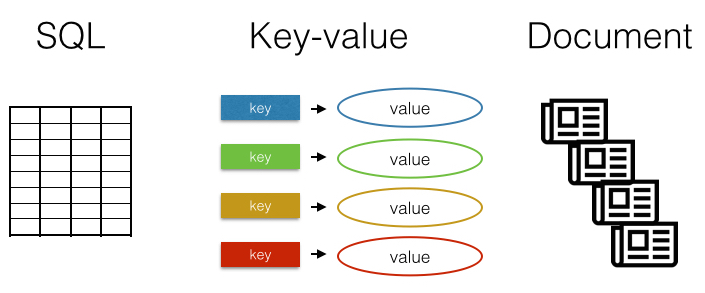
\includegraphics[width=0.8\textwidth]{key-value}
    \caption{Exemplos de estrura relacional, chave/valor e orientada a documentos}
    \label{fig:key-value}
\end{figure}
	
\subsubsection{SGBD NoSQL orientado por colunas}
	Os SGBD dessa categoria, podem ser confundidos de certa forma com um SGBD relacional por serem orientado a colunas. Mas na verdade um SGBD NoSQL orientado por colunas tem um formato híbrido entre linha e coluna. Apesar de compartilharem do conceito de armazenamento por colunas, esses SGBD não armazenam os dados em tabelas, e sim em grandes arquitetura distribuídas. Nessa categoria, cada chave é associada com uma ou mais colunas, chamada de atributos. Esse armazenamento é feito de forma que o dado seja agregado mais rapidamente e com menos processamento de entrada e saída \cite{nayak2013type}.
	
	Ou seja, esses banco de dados contém uma coluna extensível de dados fortemente relacionados, em vez de conjuntos de informação em uma estrutura rígida de tabela com linha e colunas como no modelo relacional\cite{kauremerging}. Esse tipo de NoSQL é bastante útil para operações de mineração de dados e aplicações de análise \cite{nayak2013type}. Dois grandes representantes dessa categoria são o BigTable da google \cite{Chang:2008:BDS:1365815.1365816} e o Cassandra. A figura abaixo exemplifica a diferença da estrutura orientada a colunas e orientada a documentos:
	
\begin{figure}[h]
	\centering
    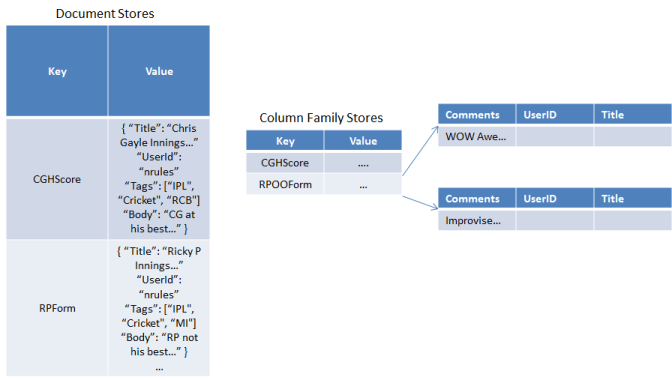
\includegraphics[width=0.8\textwidth]{columnnosql}
    \caption{Exemplo de estrutura de um NoSQL orientado a colunas.}
    \label{fig:columnnosql}
\end{figure}
	
\subsubsection{SGBD NoSQL orientado a documentos}
	Nessa categoria, os dados são armazenados em forma de documentos. Um documento dentro desse tipo de SGBD pode ser comparado a um registro dentro de um SGBD relacional, mas nos SGBD NoSQL existe uma flexibilidade maior pois é permitido uma estrutura \textit{Schema-less}. Normalmente, esses documentos seguem algum formato padrão como \textit{JSON} ou \textit{XML} por exemplo. Uma diferença com o formato dos bancos relacionais, é que um campo de um registro dentro de um SGBD relacional que não está preenchido, necessariamente ficará vazio, já num SGBD NoSQL orientado a documentos, cada documento pode ter dados similares ou não tão similares, ou seja, um campo sem informação não precisa aparecer como vazio para o usuário, demonstrando a flexibilidade que esses SGBD proporcionam \cite{nayak2013type}.
	
	Cada documento é endereçado por uma chave, da mesma forma que em SGBD NoSQL orientado a chave/valor. Esses SGBD são úteis em aplicações em que os dados não precisam ser armazenados em tabelas com campos uniformes, mas sim armazenados em documentos com características especiais. Normalmente, não é recomendado para dados com muitos relacionamentos ou normalização. Dois representantes dessa categoria são o MongoDB e o CouchDB \cite{nayak2013type}. A figura \ref{fig:columnnosql} mostra um exemplo da estrutura de um SGBD orientado a documentos em contraste com um SGBD orientado a colunas.
	
\subsubsection{SGBD NoSQL orientado a grafos}
	Nessa categoria
	
\subsubsection{SGBD NoSQL orientado a objetos}
	Nessa categoria

%%%%%%%%%%%%%%%%%%%%%%%%%%%%%%%%%%%%%%%%%%%%%%%%%%%%%%%%%%%%%%%%%%%%%%%%%%%%%%%%
%%%%%%%%%%%%%%%%%%%%%%%%%%%%%%%%%%%%%%%%%%%%%%%%%%%%%%%%%%%%%%%%%%%%%%%%%%%%%%%%
%%%%%%%%%%%%%%%%%%%%%%%%%%%%%%%%%%%%%%%%%%%%%%%%%%%%%%%%%%%%%%%%%%%%%%%%%%%%%%%%
\section{SGBD NoSQL orientado a grafos}%


%%%%%%%%%%%%%%%%%%%%%%%%%%%%%%%%%%%%%%%%%%%%%%%%%%%%%%%%%%%%%%%%%%%%%%%%%%%%%%%%
%%%%%%%%%%%%%%%%%%%%%%%%%%%%%%%%%%%%%%%%%%%%%%%%%%%%%%%%%%%%%%%%%%%%%%%%%%%%%%%%
%%%%%%%%%%%%%%%%%%%%%%%%%%%%%%%%%%%%%%%%%%%%%%%%%%%%%%%%%%%%%%%%%%%%%%%%%%%%%%%%
\section{OrientDB}

	Essa seção tem por objetivo especificar as características do SGBD OrientDB, e realizar uma comparação com outros SGBD orientado a grafos como o Neo4j.
	
\subsection{Introdução}
	
	O OrientDB, é um SGBD de código aberto sob a licensa Apache. Ele é o primeiro SGBD NoSQL multi modelo, com suporte a uma arquitetura distribuída e orientado a grafos. Sendo assim o OrientDB suporta operações com documentos, chave/valor e grafos. Essa característica garante uma enorme flexibilidade para manipular os dados dentro do OrientDB, sendo possível armazenar os dados tanto como grafos ou como documentos no mesmo banco de dados \cite{OrientDB}. A figura a seguir resume as possibilidades de registros no OrientDB:
	
\begin{figure}[h]
	\centering
    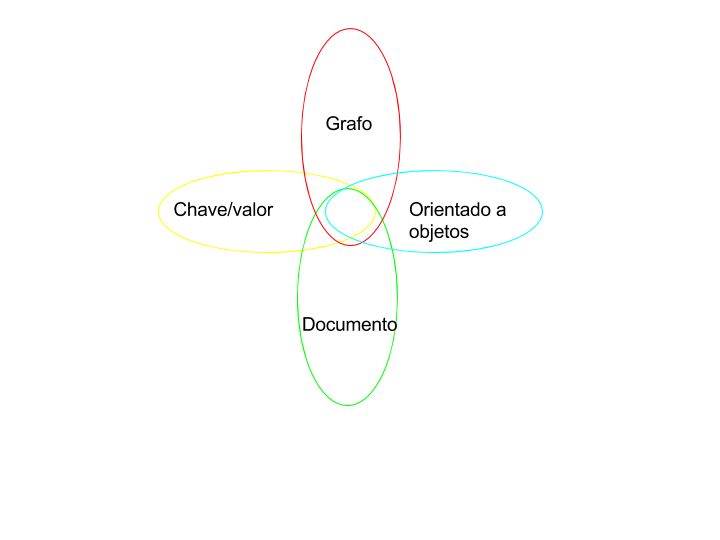
\includegraphics[width=0.8\textwidth]{orientdbmodel}
    \caption{Possibilidade de registros no OrientDB}
    \label{fig:mesh1}
\end{figure}
	
	O OrientDB é implementado utilizando a linguagem java, tendo sua primeira versão disponível no ano de 2010. Ele possui alta flexibilidade para definir o esquema do banco de dados, podendo ser \textit{Schema-free}, \textit{Schema-hybrid} ou \textit{Schema-full}. A sua linguagem de consulta é derivada do SQL o que é bastante vantajoso para aqueles que possuem experiência com bancos de dados relacionais, e além disso ele utiliza o modelo de transações ACID que como foi mencionado na seção \ref{manage_transaction} é algo mais comum no grupo dos SGBD relacionais, isso demonstra que o OrientDB presa pela integridade dos dados ao mesmo tempo que também fornece um suporte a particionamento dos dados \cite{OrientDB} \cite{vschart}.
	
	Todas essas características fazem com que o OrientDB seja um SGBD bastante flexível e confiável para se utilizar em diversas aplicações. As operações utilizando grafos em específico, vem ganhando bastante visibilidade pois funciona muito bem em certos domínios de aplicação. Como foi mencionado no capítulo \ref{chap:1} e nesse artigo feito por Matthias Gelbmann \cite{Graphpopularity} a popularidade dos SGBD orientados a grafos vem crescendo bastante nos últimos anos, e essas características ajudam a explicar o porque de banco de dados como o OrientDB e Neo4j estarem crescendo tanto em popularidade.
	
\subsection{Performance} \label{orient_performance}
	O OrientDB possui uma ótima performance em operações utilizando grafos. Um aspecto técnico que ajuda nessa qualidade é que o OrientDB trabalha cada registro como um objeto e o \textit{link} entre esses objetos não é feito por referência, e sim por \textit{link} direto. Ou seja, é salvo um ponteiro que aponta diretamente para o objeto referenciado. Isso faz com que a velocidade para recuperar informações seja muito mais rápido em comparação com os joins utilizados nos SGBD relacionais. Portanto, não existem operações de joins dentro do OrientDB para obter as relações entre os registros, sendo que ele consegue salvar certa de 120 mil registro por segundo.
	
	O OrientDB utiliza mecanismos de indexação baseados em árvores-B e hash extendido, esses mecanismos garantem uma complexidade constante para obter relacionamentos entre um registro para muitos registros. Um estudo feito pelo instituto de tecnologia de tokio e pela IBM, mostra que o OrientDB chega a ser 10 vezes mais rápido que o seu maior concorrente que é o Neo4j \cite{dayarathna2012xgdbench}.
	
\subsection{Arquitetura Distribuída}
	Em relação ao suporte a uma arquitetura distribuída, o OrientDB trabalha com um método de particionamento conhecido como \textit{sharding}, e um método de replicação conhecido como \textit{Multi-master replication}. Esse modelo de replicação, permite que qualquer membro do cluster possa ler e escrever no banco de dados. Essa arquitetura permite que exista uma escalabilidade horizontal sem gargalos, como ocorre em algumas outras soluções de SGBD NoSQL \cite{kauremerging}.
	
	No ano de 2012 o OrientDB trabalhava com uma arquitetura diferente, conhecida como \textit{Master-slave replication}. A figura a seguir exemplifica o formato dessa arquitetura.
	
\begin{figure}[h]
	\centering
    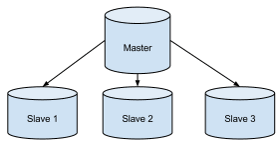
\includegraphics[width=0.5\textwidth]{master-slave}
    \caption{Exemplo de uma arquitetura \textit{Master-slave}}
    \label{fig:master-slave}
\end{figure}

	Esse tipo de arquitetura é eficiente para escalar as operações de leituras, mas também é importante conseguir escalar as operações de escrita no banco de dados. Como é possível ver na imagem acima, um nó (\textit{Master}) é responsável por receber as requisições de leitura e distribuir essa operações entre os demais nós \textit{Slaves}. Porém, ao projetar dessa forma o nó \textit{Master} se torna um gargalo para a aplicação, de forma que, ao receber muitas requisições o nó passa a ficar sobrecarregado.
	
	Uma vantagem dessa arquitetura, é sua facilidade de implementação, pois basta realizar o roteamento das requisições entre os nós \textit{Slaves}. Como desvantagens temos o fato do nó \textit{Master} ser o gargalo nas operações de escrita, e a característica de que não adianta aumentar a quantidade de servidores para aumentar a vazão, pois a vazão é inevitavelmente limitada pelo nó \textit{Master}.
	
\begin{figure}[h]
	\centering
    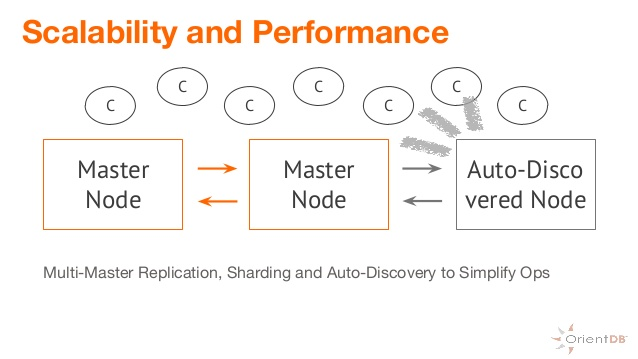
\includegraphics[width=0.5\textwidth]{orientdb-the-2nd-generation-of-multimodel-nosql-44-638}
    \caption{Exemplo de uma arquitetura \textit{Multi-master}}
    \label{fig:multi-master}
\end{figure}
	
	Nesse cenário, o SGBD evoluiu para a arquitetura \textit{Multi-master} representada pela figura acima. Nesse formato, todos os nós de um cluster aceitam operações de escrita. Além desse formato, o SGBD passou a adotar o método de particionamento conhecido como \textit{sharding}, em que os dados são divididos em múltiplas partições. Como é mencionado na seção \ref{orient_object}, o conceito de classes é bastante útil na arquitetura distribuída, uma vez que por padrão para cada classe criada o SGBD cria um cluster para que suas instâncias sejam armazenadas. Combinando essas técnicas, o OrientDB proporciona uma escalabilidade tanto em leituras quanto em escritas. Uma vantagem desse modelo é que se um nó \textit{Master} falhar, os demais podem continuar a operar normalmente.

\subsection{Orientação a Objetos} \label{orient_object}

	Uma das características mais interessantes do OrientDB é o suporte que ele da para que o usuário organize os seus dados seguindo padrões de orientação a objetos. Como foi mencionado na seção \ref{orient_performance}, o OrientDB considera cada registro como um objeto, dessa forma é possível criar classes que representam a estrutura dos dados. Por exemplo, no capítulo 3 eu explico um pouco mais sobre como fiz a modelagem dos dados seguindo o modelo MDG-NoSQL proposto por Gustavo C. Galvão Van Erven\cite{mdgnosql}. Nessa modelagem eu identifiquei as seguintes classes Transação, Empresa fornecedora, Parlamentar e Pessoa. O OrientDB permite que eu crie essas classes e ao inserir um vértice eu especifique que esse vértice é de uma classe específica, isso facilita bastante na hora de escrever as consultas pois basta utilizar o nome da classe que todos os vértices pertencentes a essa classe serão obtidos. O conceito de classe também se aplica as arestas, e tudo isso facilita na organização dos dados e na escrita de consultas ao banco de dados.
	
	Um registro é a menor unidade que é possível salvar e obter no banco de dados do OrientDB, ele pode ser obtido de quatro formas:
	
	\begin{itemize}
		\item Documento
		\item \textit{RecordBytes} (BLOB)
		\item Vértice
		\item Aresta
	\end{itemize}
	
	Dessa forma, uma classe para esse tipo de registro, é o conceito mais próximo de tabela existente no OrientDB. O conceito de herança, muito utilizado no paradigma orientado a objetos, também possui suporte no OrientDB, sendo que classes podem herdar atributos e propriedades de uma classe pai. Por exemplo, a classe pessoa mencionada acima, pode ser a classe pai da classe parlamentar, assim um parlamentar herda atributos de pessoa. Além disso, ao realizar uma consulta utilizando a classe pessoa, automaticamente todos os parlamentares também serão utilizados. Outra funcionalidade atrelada a esse assunto, é o suporte a classes abstratas utilizadas para definir outras classes. Uma classe abstrata não possui instâncias no banco de dados, bastante similar com os conceitos em orientação a objetos. 
	
	A figura a seguir exemplifica a herança presente no OrientDB, no caso é possível criar três classes para armazenar as instâncias dos vértices, que são: \textit{Employee}, \textit{Regular employee} e \textit{Contract employee}. As duas últimas classes herdam os atributos id e name da classe pai, sendo que ao realizar uma busca por todos as instâncias de \textit{Employee}, tanto \textit{Regular employee} quanto \textit{Contract employee} serão retornados.
	
\begin{figure}[h]
	\centering
    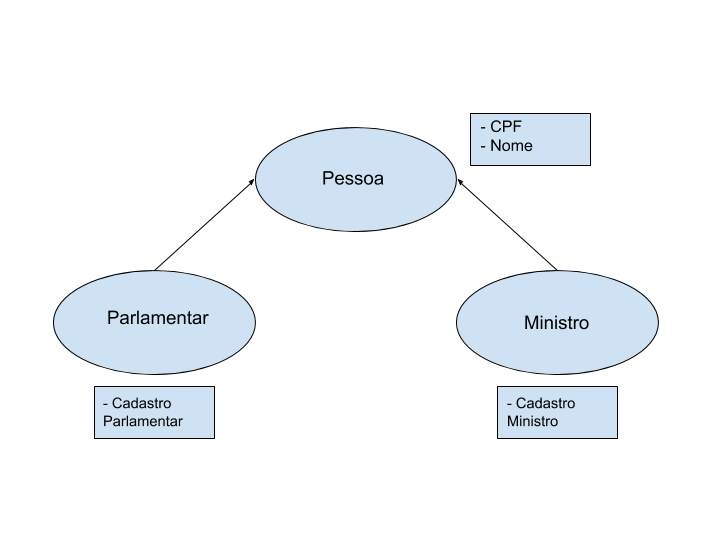
\includegraphics[width=0.5\textwidth]{teleporter-inheritance-orientdb-schema}
    \caption{Exemplo de herança no \textit{schema} do OrientDB }
    \label{fig:mesh1}
\end{figure}
	
	Para finalizar é importante mencionar que as classes tem um papel importante ao se utilizar a arquitetura distribuída no OrientDB, pois para cada classe criada, o SGBD cria um cluster automaticamente para armazenar instâncias dessas classes. Essa funcionalidade auxilía bastante na organização do particionamento dos dados em um ambiente distribuído. Todos os registros de uma classe são armazenados juntos no mesmo cliuster que tem o mesmo nome da classe. No OrientDB é possível criar até trinta e dois mil setecentos e setenta e sete clusters. Compreender bem os conceitos de classes nesse SGBD, permite que o usuário tenha vantagem ao fazer o \textit{design} do banco de dados. Vale lembrar que uma classe pode ser mapeada para n clusters como mostra a figura a seguir:
\begin{figure}[h]
	\centering
    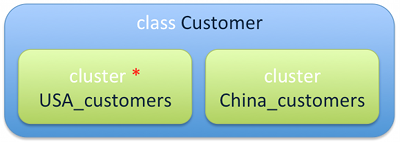
\includegraphics[width=0.5\textwidth]{class-clusters}
    \caption{Classe Customer mapeada para dois clusters diferentes}
    \label{fig:mesh1}
\end{figure}

%%%%%%%%%%%%%%%%%%%%%%%%%%%%%%%%%%%%%%%%%%%%%%%%%%%%%%%%%%%%%%%%%%%%%%%%%%%%%%%%
%%%%%%%%%%%%%%%%%%%%%%%%%%%%%%%%%%%%%%%%%%%%%%%%%%%%%%%%%%%%%%%%%%%%%%%%%%%%%%%%
%%%%%%%%%%%%%%%%%%%%%%%%%%%%%%%%%%%%%%%%%%%%%%%%%%%%%%%%%%%%%%%%%%%%%%%%%%%%%%%%
\section{REST}


%%%%%%%%%%%%%%%%%%%%%%%%%%%%%%%%%%%%%%%%%%%%%%%%%%%%%%%%%%%%%%%%%%%%%%%%%%%%%%%%
%%%%%%%%%%%%%%%%%%%%%%%%%%%%%%%%%%%%%%%%%%%%%%%%%%%%%%%%%%%%%%%%%%%%%%%%%%%%%%%%
%%%%%%%%%%%%%%%%%%%%%%%%%%%%%%%%%%%%%%%%%%%%%%%%%%%%%%%%%%%%%%%%%%%%%%%%%%%%%%%%